\externaldocument{text-02-teoreticka}
\subsection{Koncept identifikace nejlepší nosnice}\label{subsec:koncept-identifikace-nejlepsi-nosnice}

Při chovu slepic by bylo velmi užitečné vědět, kolik vajec která slepice snáší, protože to umožňuje farmáři sledovat produktivitu jednotlivých slepic.
Díky tomu může:
\begin{itemize}
    \item Optimalizovat chov: Identifikací slepic s vysokou a nízkou snáškou může farmář rozhodnout o selekci nebo o zvláštní péči pro méně produktivní slepice.
    \item Zlepšit zdraví slepic: Nízká snáška může být indikátorem zdravotních problémů. Včasná identifikace umožňuje podniknout kroky k léčbě nebo prevenci nemocí.
    \item Efektivněji plánovat krmení a zdroje: Sledování výkonu pomáhá v rozhodování o výživě a péči, aby byla maximalizována produkce vajec při optimálních nákladech.
    \item Zvýšit ziskovost: Monitorováním snášky lze zlepšit celkovou produktivitu farmy a tím i její ekonomickou efektivitu.
\end{itemize}

Celkově tedy znalost počtu vajec od každé slepice pomáhá v efektivním řízení chovu a zajišťuje lepší výsledky jak po stránce produkční, tak ekonomické.
Abych toho dosáhl, potřebuji být schopen jednotlivé slepice identifikovat a tuto informaci propojit s momentum, kdy slepice sense v kurniku vejce.
V sekci  pridat odkaz  “Vaha”, je popsan mechanismus, kdy pravidelnou analyzou casove rady, kterou poskytuje vaha ziskame informaci o casove udaji, kdy bylo vejce sneseno.
Pak jiz jen staci identifikovat, ktera z nasich slepic byla v tu dobu v hnízdě.
Existuje několik variant, jak slepice identifikovat, já jsem se rozhodl využít k identifikaci obrazovou analýzu.
Postupuji následujícím způsobem.
Nejprve procházím videozáznam a identifikuji oblasti, kde se slepice nacházejí.
Tyto oblasti následně vystřihnu a uložím do samostatných souborů.
Poté procházím tyto menší obrázky a pomocí segmentace vystřihnu plochu, kde je slepice, zatímco ostatní části zůstanou bílé.
Takto vyříznuté obrázky převádím na tenzory.
Převod na tenzor znamená, že dvourozměrný obraz (matice pixelů) převedu do vícerozměrné datové struktury, která dokáže reprezentovat různé vlastnosti obrazu a je vhodná pro strojové učení a další matematické zpracování.
Tímto způsobem získám numerickou reprezentaci obrazu, se kterou mohu efektivně pracovat.
Získané tenzory porovnávám se vzorovými vektory uloženými v databázi.
Pokud je vektor shodný, znamená to, že jsem našel odpovídající slepici, a podařilo se mi ji tak identifikovat.

Algoritmus tedy na počátku vezme jako vstup obrázek z kamery viz obrázek~\ref{fig:source_chick_image}.
Dále je obrázek segmentován a jsou vyjmuty pouze tvary, které algoritmus vyhodnotil jako slepice viz obrázek~\ref{fig:segmented_chicks2}.
Na závěr je pro každý výřez vypočítán tenzor na jehož základě jsou slepice roztřízeny do jednotlivých skupin podle barvy viz obrázek~\ref{fig:chicks_in_clusters}.



\begin{figure}[h]
    \centering
    \begin{subfigure}[t]{1\textwidth}
        \centering
        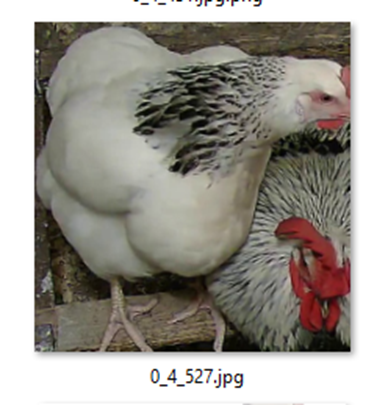
\includegraphics[width=\textwidth]{img/source_chick_image}
        \caption{Jeden ze vstupů do algoritmu pro nosnice}
        \label{fig:source_chick_image}
    \end{subfigure}

    \begin{subfigure}[t]{1\textwidth}
        \centering
        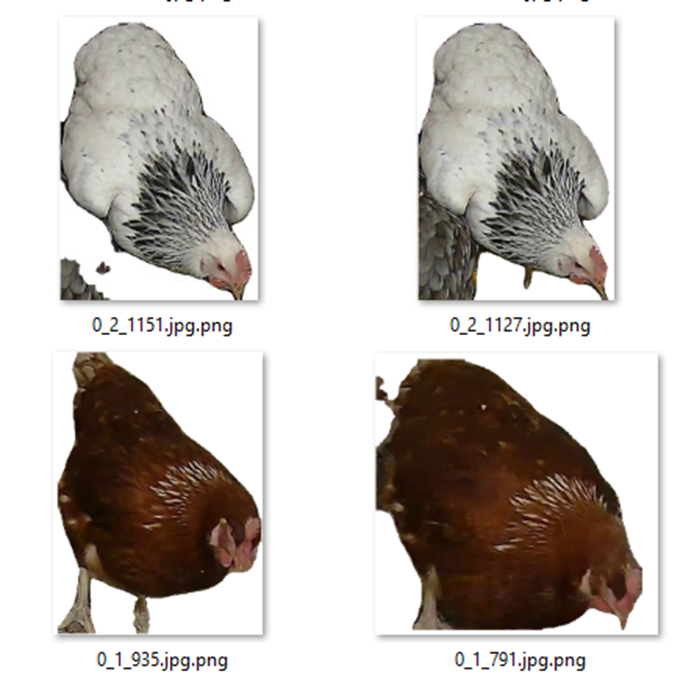
\includegraphics[width=\textwidth]{img/segmented_chicks}
        \caption{Segmentované slepice z fotek}
        \label{fig:segmented_chicks2}
    \end{subfigure}

    \begin{subfigure}[t]{1\textwidth}
        \centering
        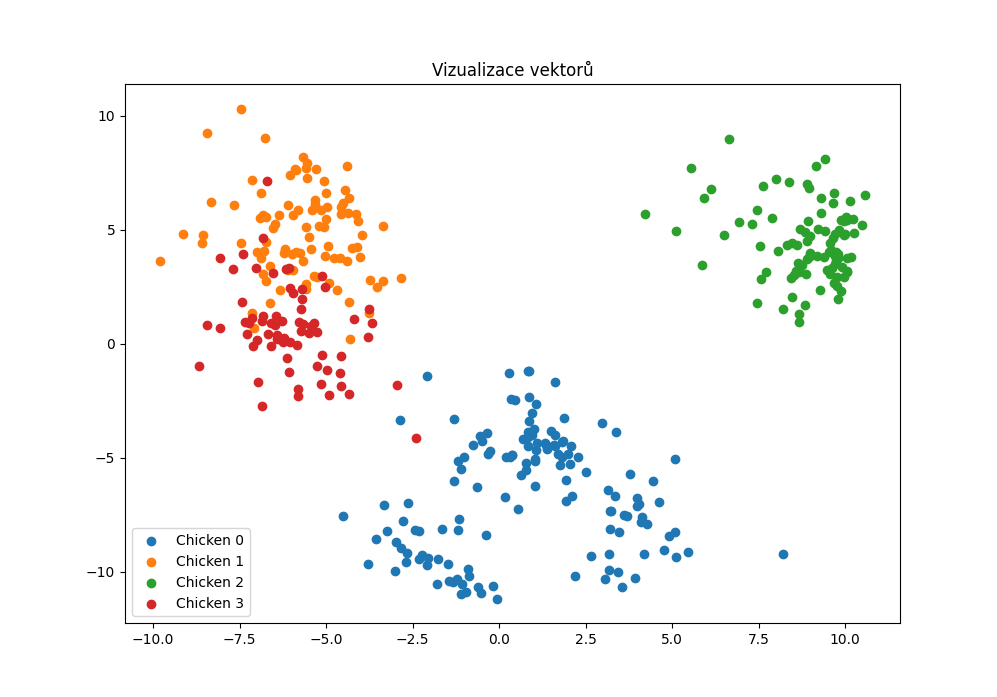
\includegraphics[width=\textwidth]{img/chicks_in_clusters}
        \caption{Algoritmem rozdělené slepice dle tenzorů}
        \label{fig:chicks_in_clusters}
    \end{subfigure}
\end{figure}
